%% LyX 2.3.0 created this file.  For more info, see http://www.lyx.org/.
%% Do not edit unless you really know what you are doing.
\documentclass[a4paper,english]{article}
\usepackage[T1]{fontenc}
\usepackage[utf8x]{inputenc}
\setlength{\parindent}{0bp}
\usepackage{graphicx}

\makeatletter

%%%%%%%%%%%%%%%%%%%%%%%%%%%%%% LyX specific LaTeX commands.
\pdfpageheight\paperheight
\pdfpagewidth\paperwidth

%% A simple dot to overcome graphicx limitations
\newcommand{\lyxdot}{.}


%%%%%%%%%%%%%%%%%%%%%%%%%%%%%% User specified LaTeX commands.
% used packages
\usepackage[margin=1in]{geometry}
\usepackage[utf8x]{inputenc}
\usepackage{afterpage}
\usepackage{xcolor}
\usepackage{pdfpages}
\usepackage{graphicx}
\usepackage{caption}

\usepackage{expl3}
\expandafter\def\csname ver@l3regex.sty\endcsname{}
\usepackage{coloremoji}

\usepackage[outputdir=./tmp,newfloat]{minted} % need to call 
%<pdflatex -shell-escape>

%% by overleaf %%
\usepackage{listings}
%New colors defined below
\definecolor{codegreen}{rgb}{0,0.6,0}
\definecolor{codegray}{rgb}{0.5,0.5,0.5}
\definecolor{codepurple}{rgb}{0.58,0,0.82}
\definecolor{backcolour}{rgb}{0.95,0.95,0.92}
%Code listing style named "mystyle"
\lstdefinestyle{mystyle}{
	backgroundcolor=\color{backcolour},
	commentstyle=\color{codegreen},
	keywordstyle=\color{magenta},
	numberstyle=\tiny\color{codegray},
	stringstyle=\color{codepurple},
	basicstyle=\ttfamily\footnotesize,
	breakatwhitespace=false,         
	breaklines=true,                 
	captionpos=b,                    
	keepspaces=true,                 
	numbers=left,                    
	numbersep=5pt,                  
	showspaces=false,                
	showstringspaces=flase,
	showtabs=false,                  
	tabsize=2
}
%"mystyle" code listing set
\lstset{style=mystyle}


\usepackage{fancyhdr}
\pagestyle{fancy}
\fancyhf{} 	% it clears the header and footer of default "plain" page style
\lhead{\leftmark}
\rhead{\thepage}
\chead{\hyperlink{Contents}{Contents}}

\usepackage{hyperref}
\hypersetup{
	colorlinks=true,
	linkcolor=orange,
	urlcolor=magenta
}

\@ifundefined{showcaptionsetup}{}{%
	\PassOptionsToPackage{caption=false}{subfig}}
\usepackage{subfig}
\AtBeginDocument{
	\def\labelitemii{}
}

\makeatother


\linespread{1.1}
\setlength{\parindent}{0bp}

\usepackage{babel}
\begin{document}
	% cover page
	\thispagestyle{empty}
	\begin{figure}
		\centering
		
\includegraphics[width=1.0\linewidth]{img/lion.png}
		\caption*{\href{https://github.com/How-u-doing}{how U doin'?}
			\\ $🐊^{🐊^{🐊}} = ∫_{🎃}^{🎅} 🙊 \ d🍀$ }
		\label{cover:lion}
	\end{figure}
	\pagecolor{pink}
	\afterpage{\nopagecolor}
	\clearpage
	\newpage
	
	\title{Modeling hw4\thanks{This article was typeset by Mark Taylor using 
	the \protect\LaTeX{}
			document processing system. }}
	
	\author{10170437 Mark Taylor}
	
	\date{May 27, 2020}
	
	\maketitle
	
	\phantomsection 
	\hypertarget{Contents}{}  % Make an anchor to the toc
	\tableofcontents
	
	\section{Problems}
	
	\begin{figure}[!hb]
		\centering
		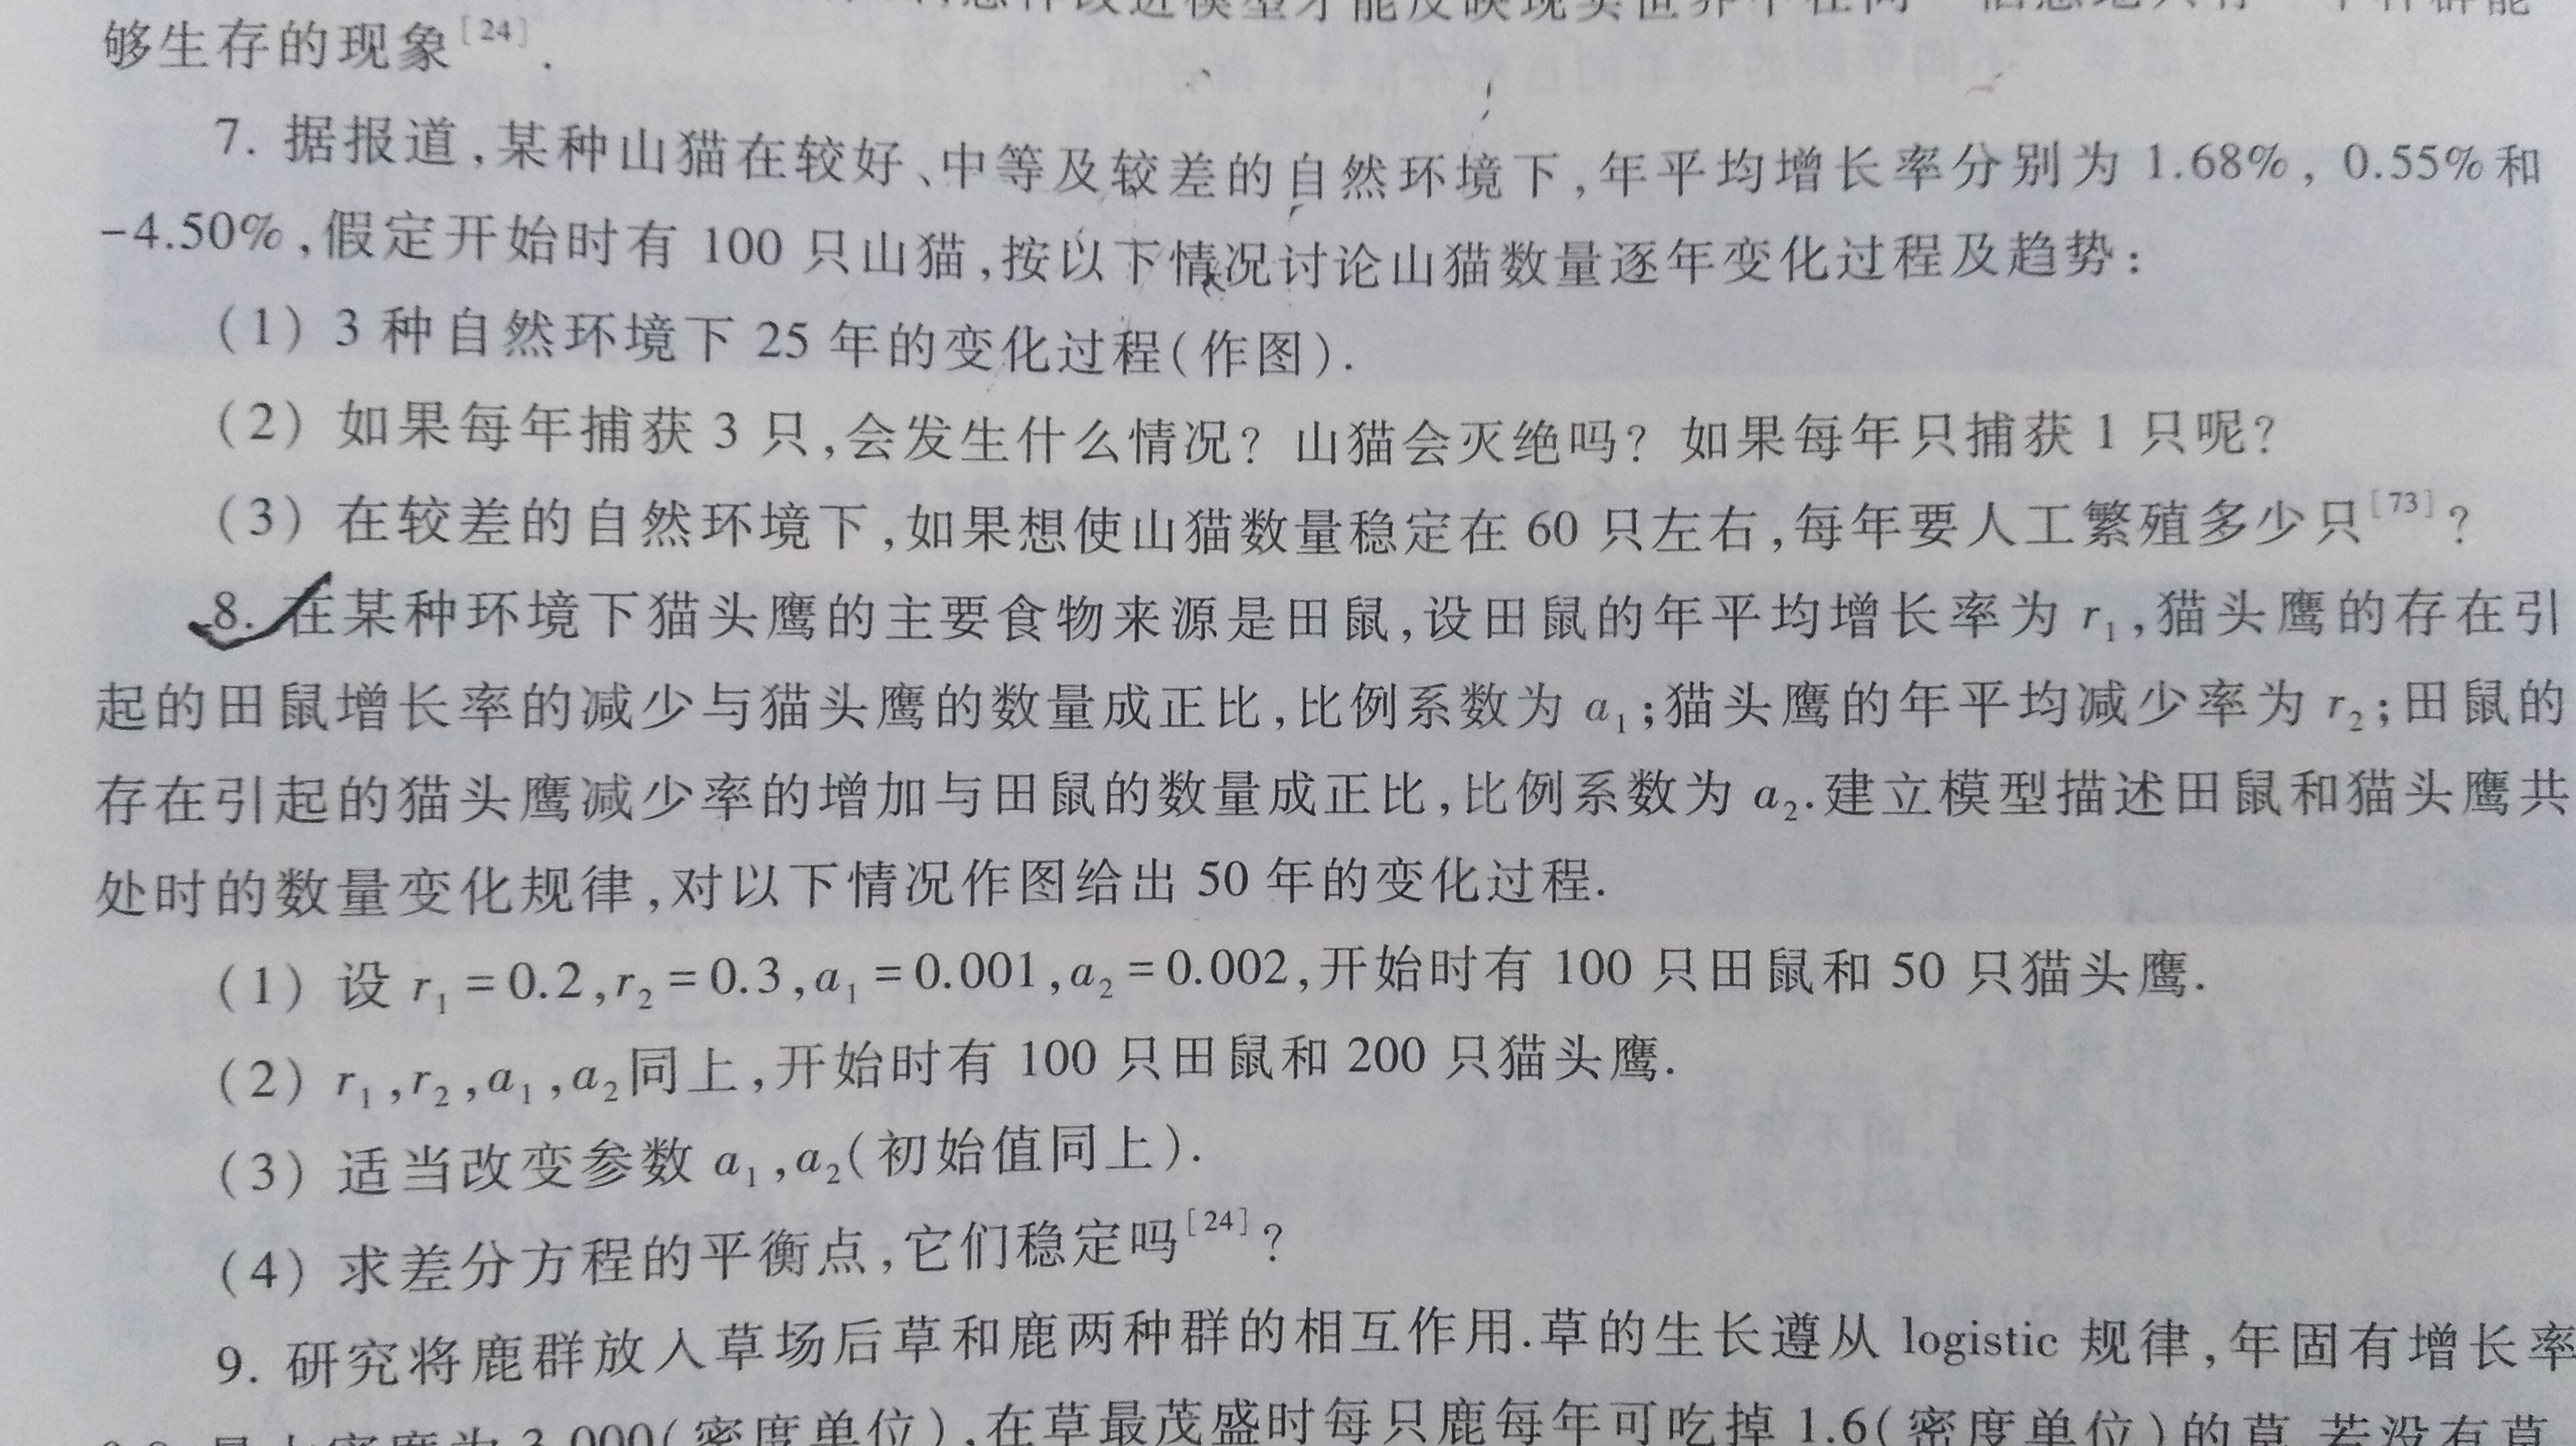
\includegraphics[width=1.0\linewidth]{img/problem}
		\caption*{}
		\label{fig:problem}
	\end{figure}
	
	\section{Model Establishing}
	Let $x_k, y_k$ be number of rats \& owls in the $k$th year respectively. 
	By observing the problem, 
	we can obtain following difference equations. 
	$$
	x_{k+1}=(1+r_1-a_1 y_k ) x_k,
	$$$$  
	y_{k+1}=(1-r_2+a_2 x_k ) y_k.
	$$
	
	\section{Questions }
	
	❓ ❓ ❓ 
	\renewcommand{\labelenumi}{\roman{enumi}}
	\begin{enumerate} 
		\item  Let $r_1=0.2,r_2=0.3,a_1=0.001,a_2=0.002$, with 100 rats and 50 
		owls in the beginning. 
		\item  With 100 rats and 200 owls in the beginning, and coefs are the 
		same as (i).
		\item  Change the arguments aptly (with the same initial values in 
		(ii)).
		\item  Solve the equilibrium point. Does it stable? 
	\end{enumerate}
	
	\section{Solutions}
	
	🔑 🔑 🔑 \\[5pt]
	Let's first determine the equilibrium point (question 4), let it be 
	$E=(\alpha,\beta)$.
	By the concept, when it goes stable, we have $x_k \rightarrow x_{k+1}, y_k 
	\rightarrow y_{k+1} as k \rightarrow $,
	i.e. $\frac{x_k}{x_{k+1}}\rightarrow 1,\frac{y_k}{y_{k+1}}\rightarrow 1$. 
	Thus we have,
	$$
	1=1+r_1-a_1 y_k, $$$$
	1=1-r_2+a_2 x_k,
	$$
	which indicate $\alpha=\frac{r_1}{a_1}=200$ and 
	$\beta=\frac{r_2}{a_2}=150$. Therefore, $E=(200,150)$. 
	\par
	Let’s do a little programming to draw these graphs. In this section, we 
	will see those graphs rendered.
	
	\begin{figure}[!hb]
		\makebox[\textwidth][c]{
			
			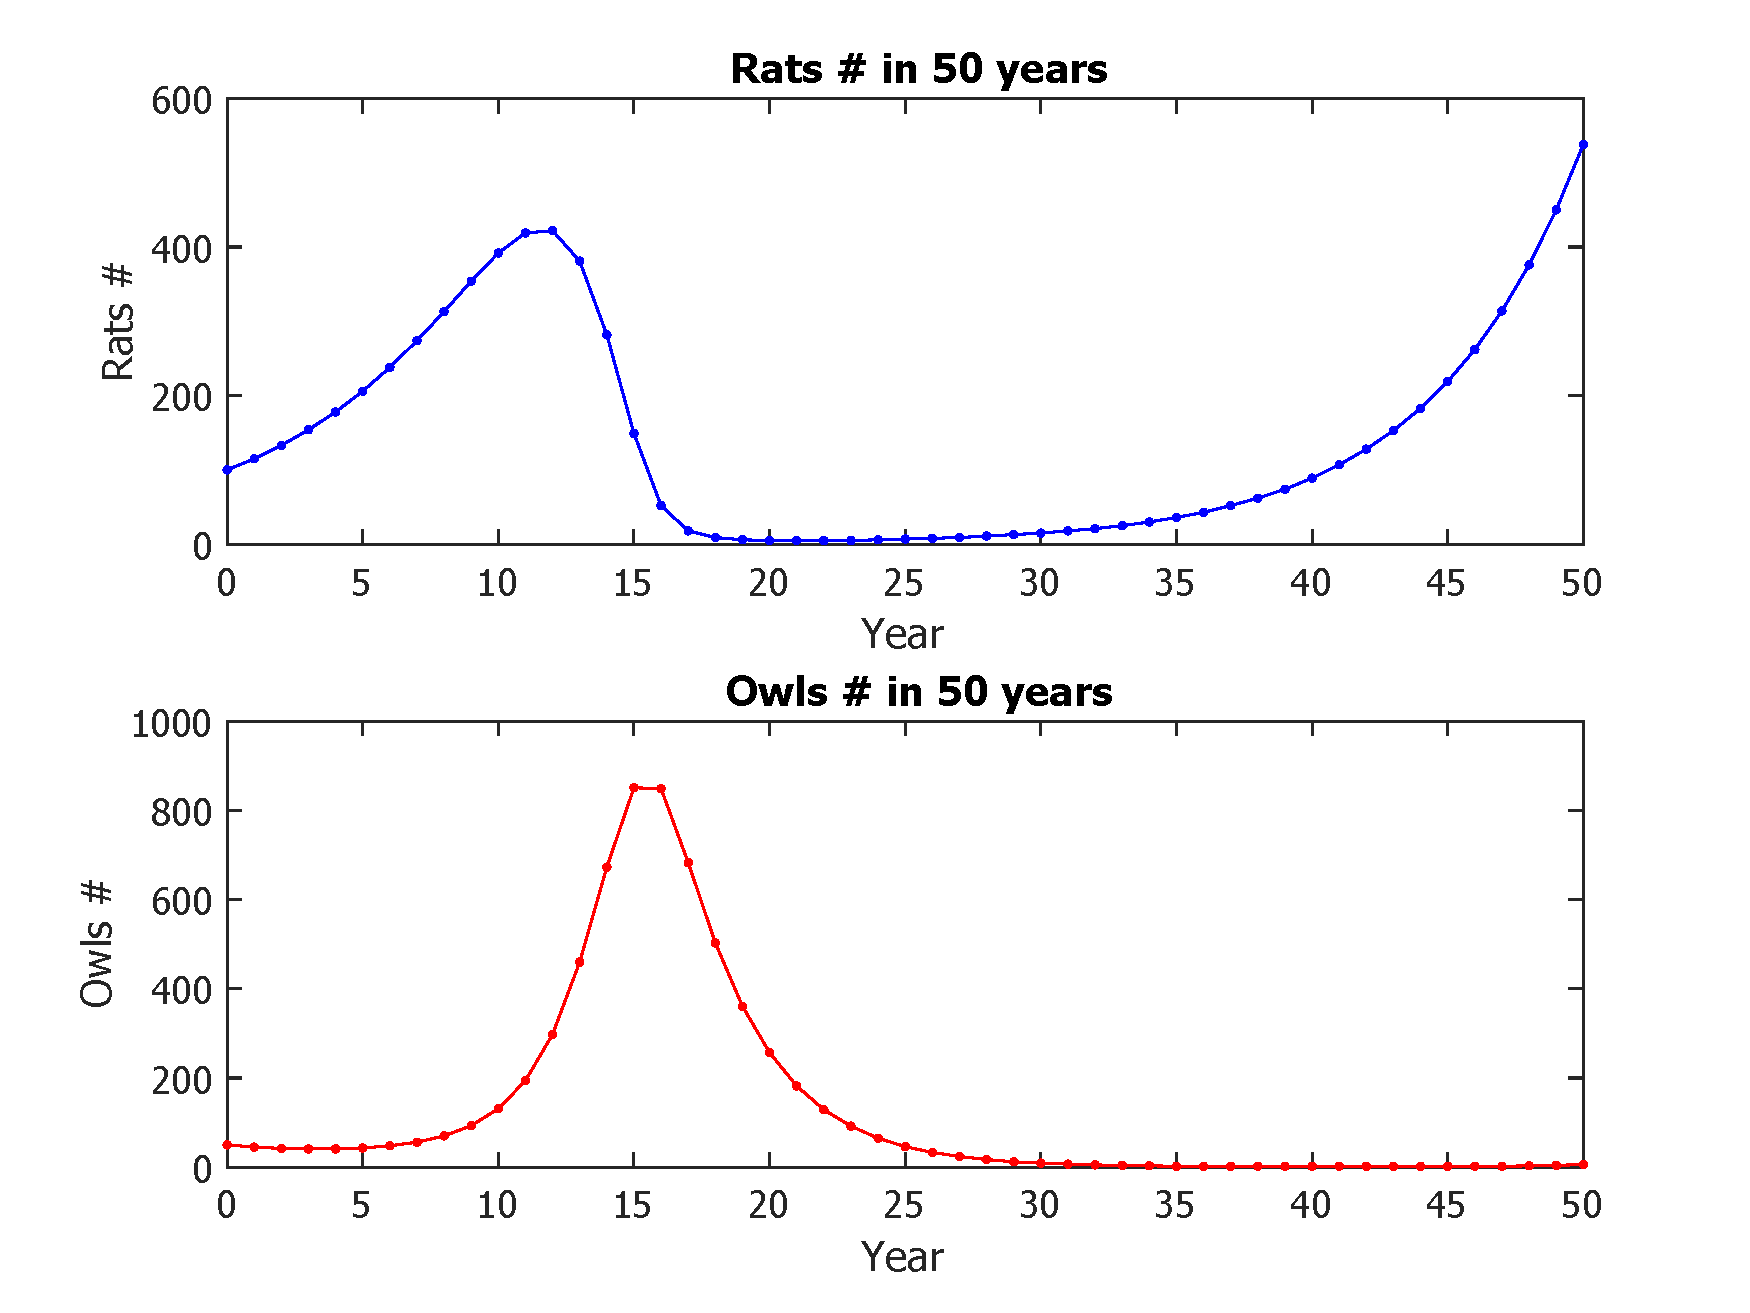
\includegraphics[width=0.47\paperwidth]{svg/ques_1_subplot}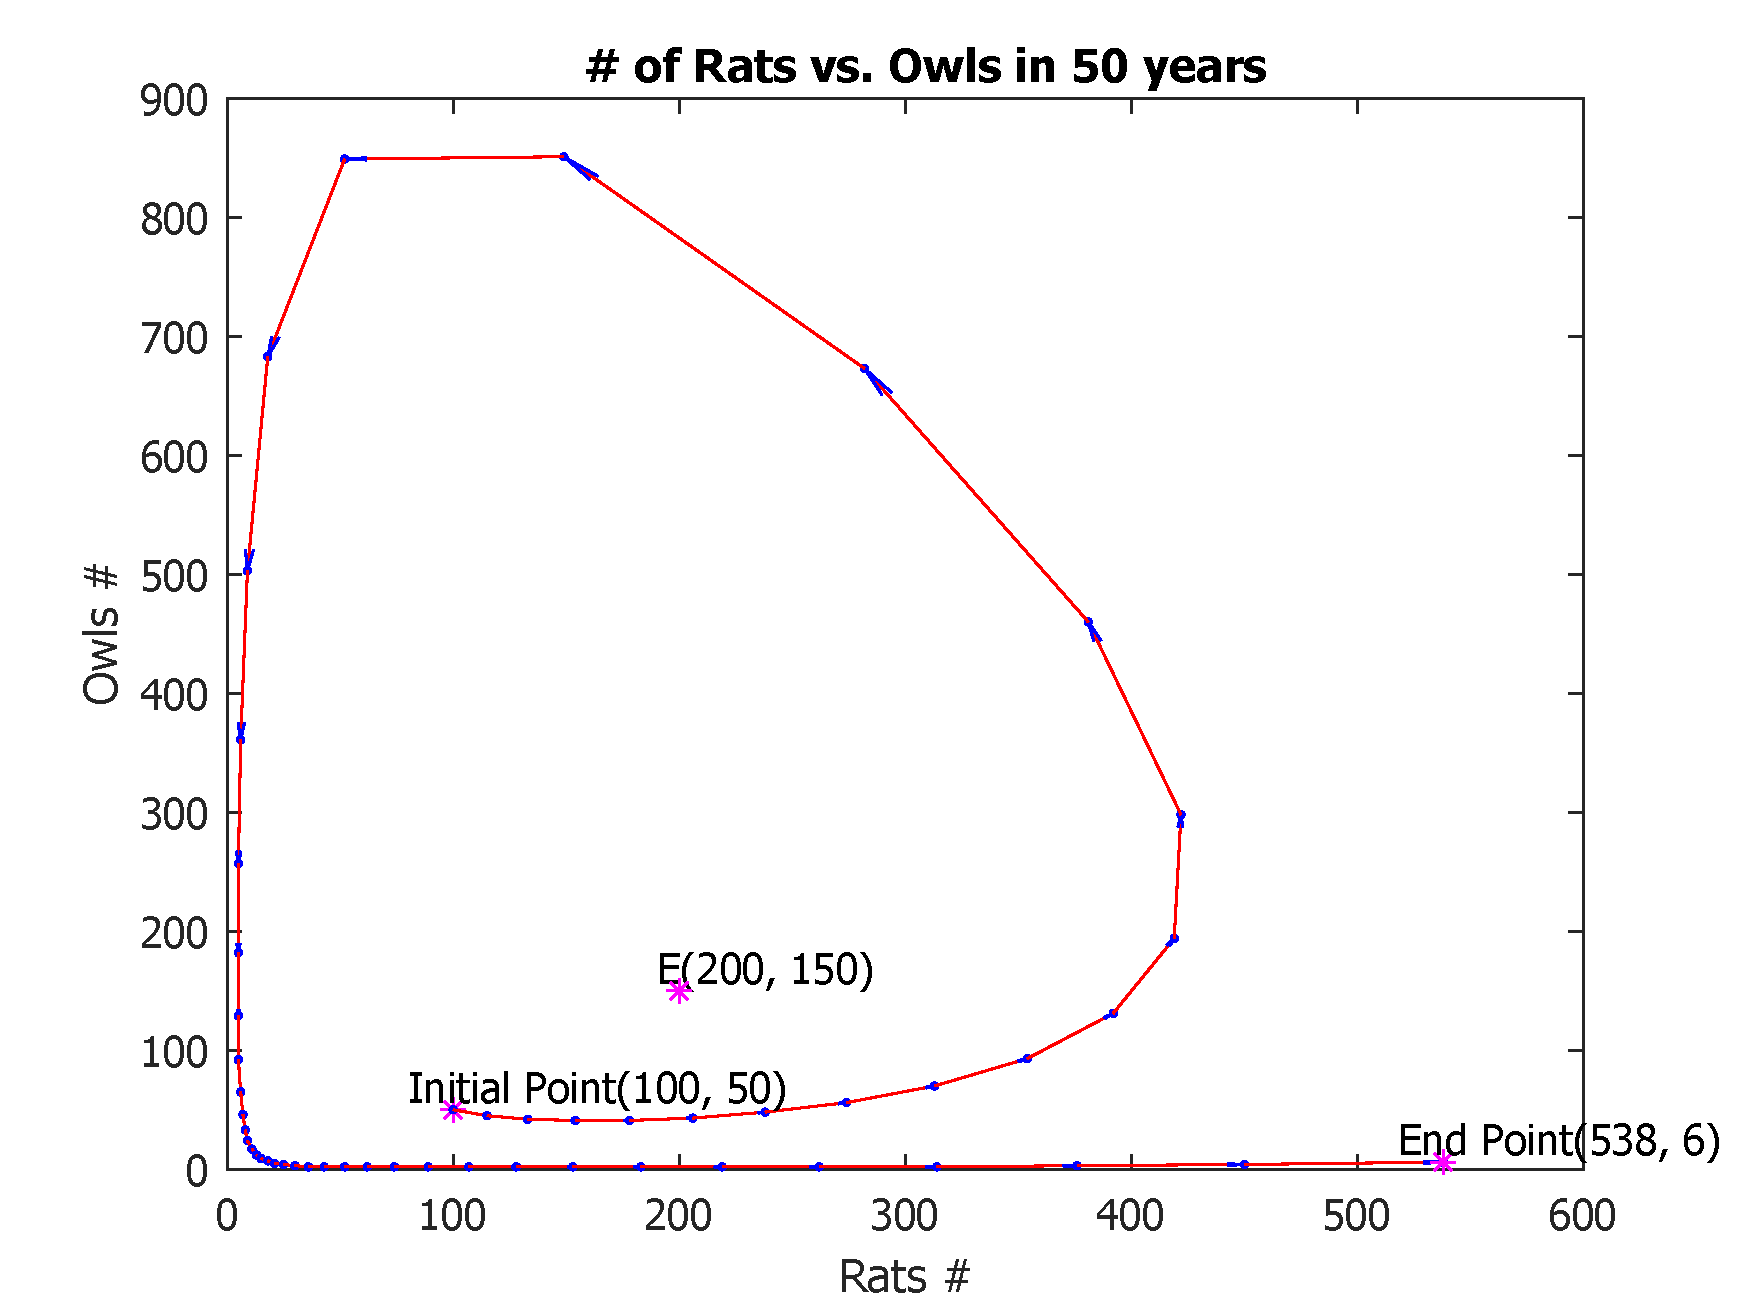
\includegraphics[width=0.47\paperwidth]{svg/ques_1_relationship}}\caption{Question
			 1\label{fig:Question-1}}
	\end{figure}
	
	See code of question 1, 2, \& 4 \hyperref[exer8_q124_helper]{here💻}
	
	
	\clearpage
	And the following graphs are by question 2.
	
	\begin{figure}[!hb]
		\makebox[\textwidth][c]{
			
			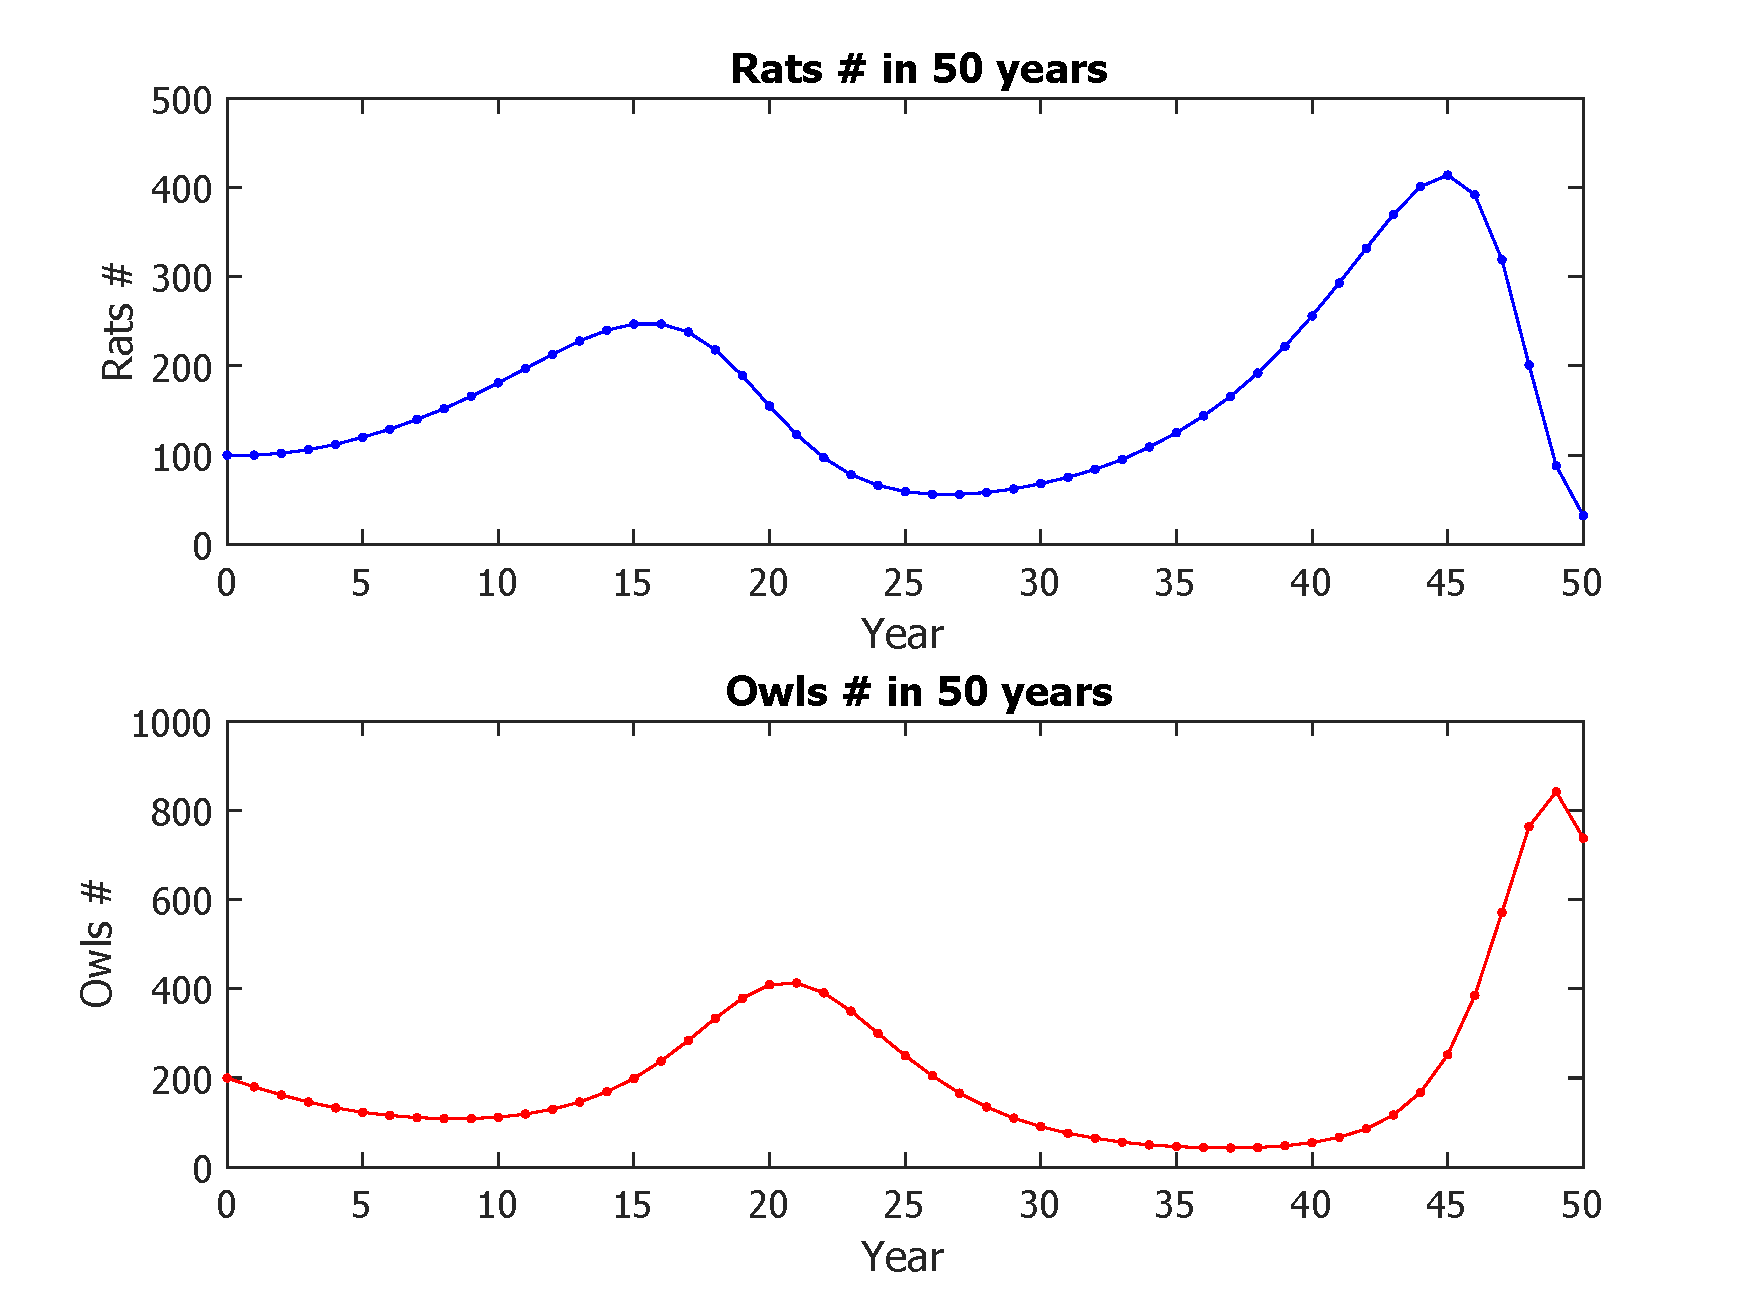
\includegraphics[width=0.47\paperwidth]{svg/ques_2_subplot}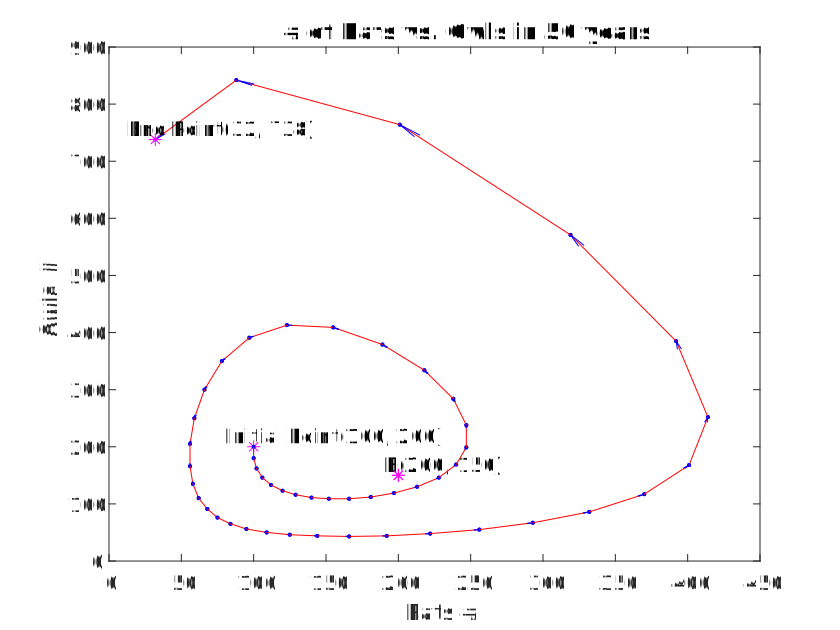
\includegraphics[width=0.47\paperwidth]{svg/ques_2_relationship}}
		
		\caption{Question 2\label{fig:Question-2}}
	\end{figure}
	
	In question 3, we plot a dynamic graph, you can run these \emph{MATLAB}
	programs in the \emph{src }folder and see how it changes. View code
	\hyperref[exer8_q3_helper]{here💻}.\\
	
	Note that we let $a_{1}$ \& $a_{2}$ satisfy some (reasonable) relationship,
	say $a_{2}=\frac{a_{2}+0.003}{a_{1}+0.001}*a_{1}$. (???) Then change
	$a_{1}$ by a vector.\\
	\begin{figure}
		\makebox[\textwidth][c]{
			
			\subfloat[$a_{1}=0.0012$, 
			$a_{2}=0022$]{\includegraphics[width=0.47\paperwidth]{svg/ques_3_0\lyxdot
			 0012_0\lyxdot 0022}}\subfloat[$a_{1}=0.0015$, 
			$a_{2}=0027$]{\includegraphics[width=0.47\paperwidth]{svg/ques_3_0\lyxdot
			 0015_0\lyxdot 0027_(100_years)}
				
		}}\\
		
		\makebox[\textwidth][c]{
			
			\subfloat[$a_{1}=0.0016$, 
			$a_{2}=0029$]{\includegraphics[width=0.47\paperwidth]{svg/ques_3_0\lyxdot
			 0016_0\lyxdot 0029}
				
			}\subfloat[$a_{1}=0.0021$, 
			$a_{2}=0035$]{\includegraphics[width=0.47\paperwidth]{svg/ques_3_0\lyxdot
			 0021_0\lyxdot 0035}
				
			}
			
		}
		
		\caption{Question 3\label{fig:Question-3}}
	\end{figure}
	
	Finally, we get into question 4, the last one. We shall enlarge the
	time span so that we can see whether the graph is converging to
	a specific point (the equilibrium point $E$ ) or diverging away form
	the equilibrium point. \\[5pt]
	
	We can see that each of these figures suggests that it's \textbf{NOT 
	stable}.
	\begin{figure}
		\makebox[\textwidth][c]{
			
			\subfloat[Plot of rats \# \& owls \# in 200 years respectively 
			]{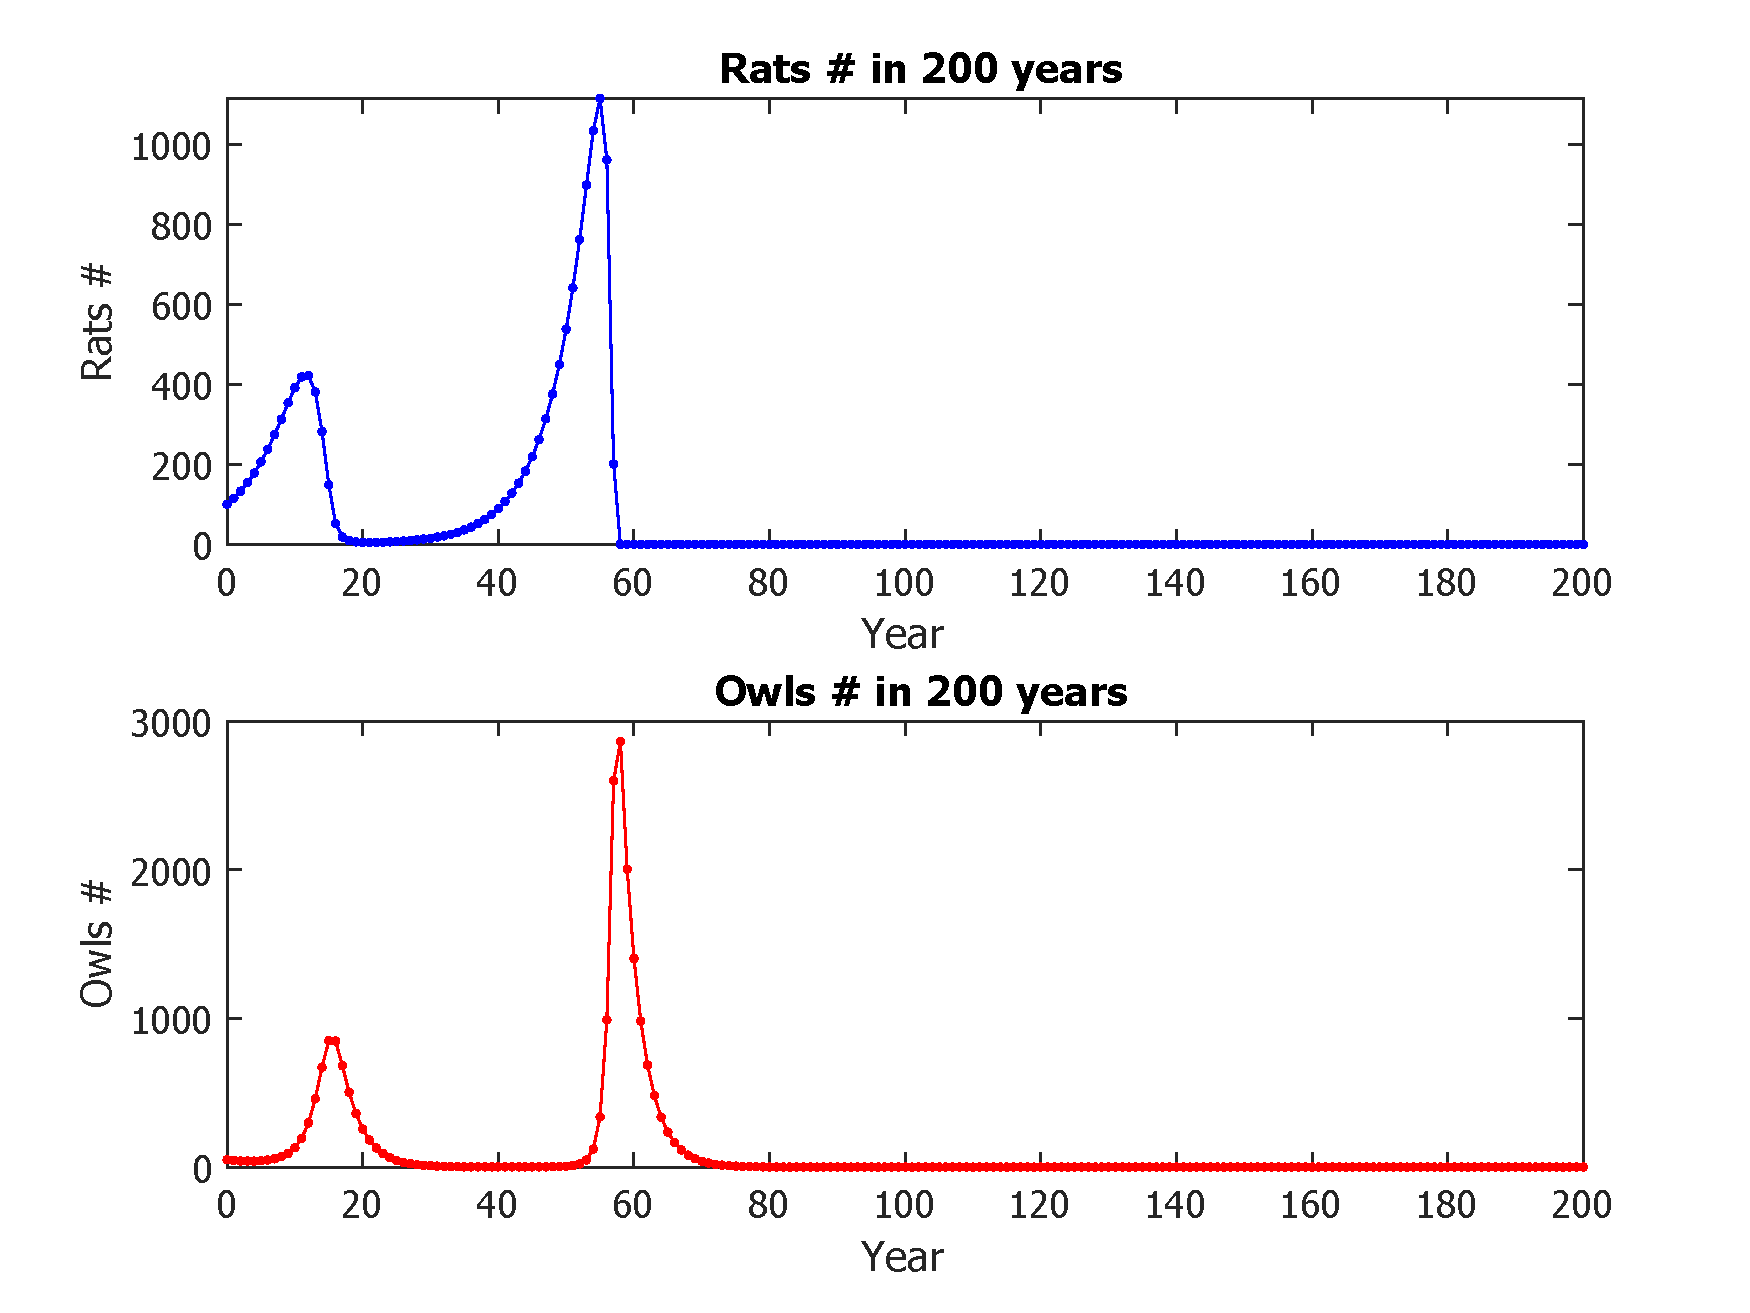
\includegraphics[width=0.8\paperwidth]{svg/ques_4_subplot}}
			
		}\\
		
		\makebox[\textwidth][c]{
			
			\subfloat[\# of rats vs. owls in 200 
			years]{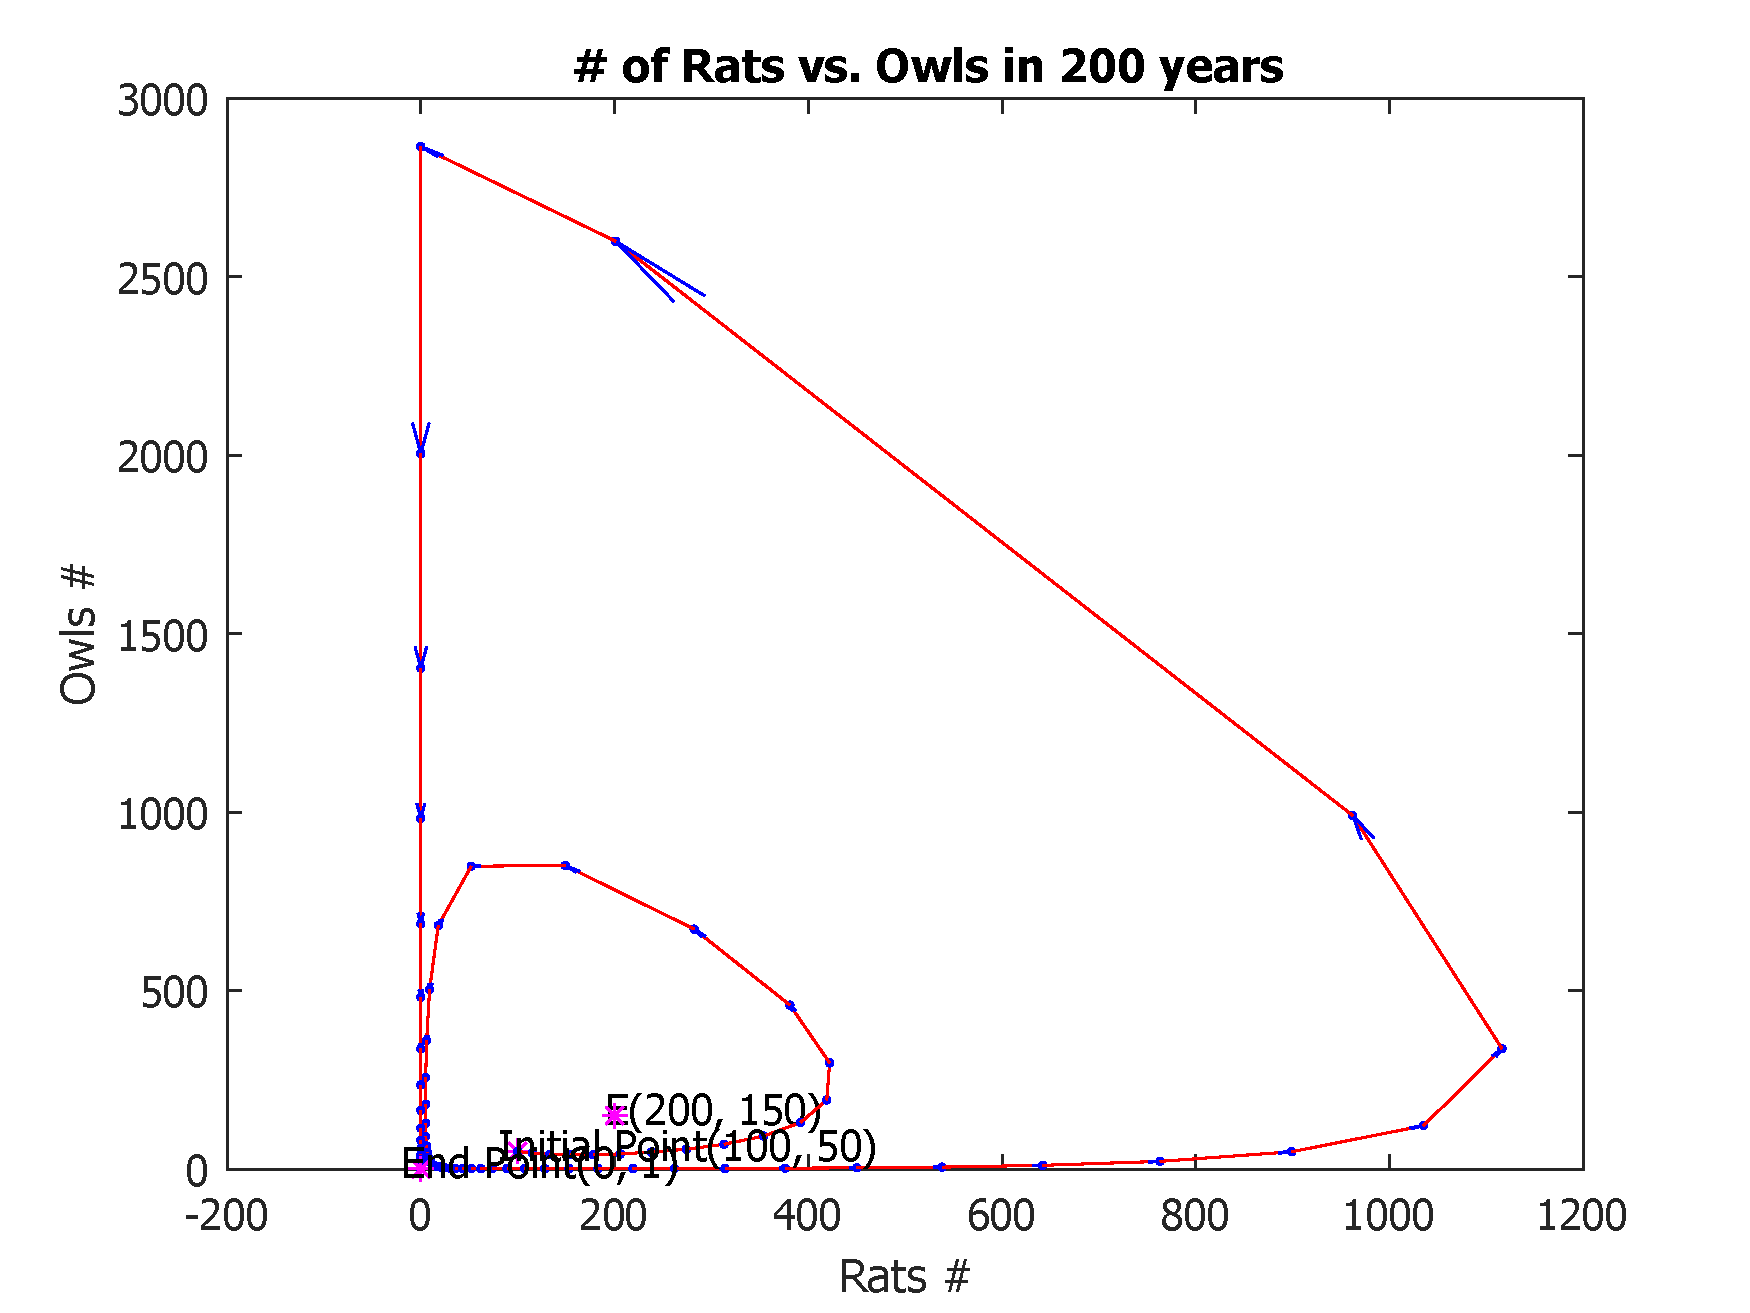
\includegraphics[width=0.49\paperwidth]{svg/ques_4_relationship}}\subfloat[Roomed
			 in graph of 
			(b)]{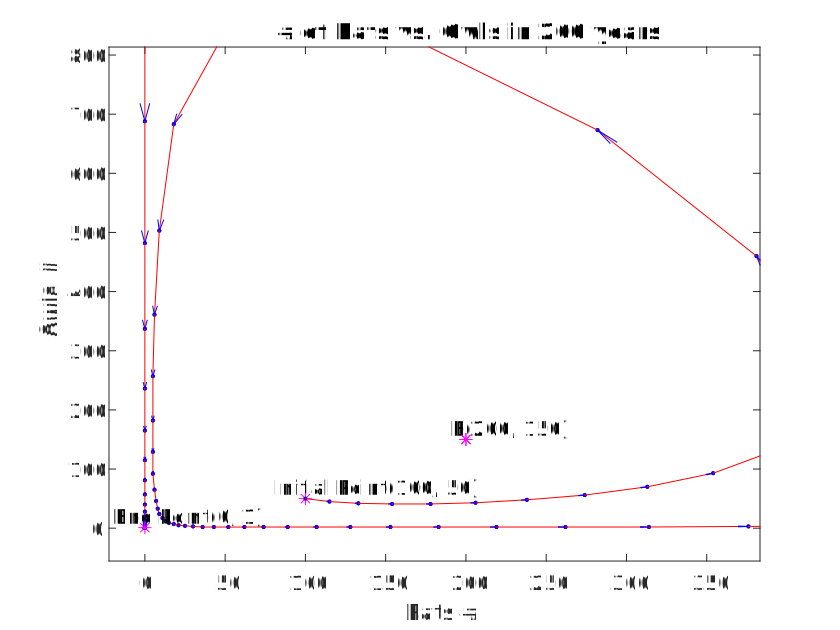
\includegraphics[width=0.49\paperwidth]{svg/ques_4_relationship_roomed_in}
				
			}
			
		}\caption{Question 4\label{fig:Question-4}}
	\end{figure}
	
	
	\clearpage 
	\section{Code}
	
	\subsection{main function}
	
	This is the main function that calls other auxiliary functions that
	serve as modules. 
	
	%\begin{listing}[ht]
	%	\inputminted{octave}{src/exer8_main.m}
	%	\caption{main function for solving exercise 8}
	%	\label{exer8_main}
	%\end{listing}
	
	\lstinputlisting[language=Octave, 
	caption={Main function for solving exercise 8.},
	label=exer8_main
	]{src/exer8_main.m}
	
	\subsection{exer8\_q124\_helper}
	This is an auxiliary function that solves question 1, 2, \& 4. See
	also graphs of question {\hyperref[fig:Question-1]{1}, 
		\hyperref[fig:Question-2]{2}, \hyperref[fig:Question-4]{4}.}
	\lstinputlisting[language=Octave, 
	caption={Helper function for solving question 
		{\hyperref[fig:Question-1]{1}}, % NOTE that within a list [], using 
		%hyperref will also use [], so to escape it, we need one more {}
		{\hyperref[fig:Question-2]{2}}, \& {\hyperref[fig:Question-4]{4}}.} ,
	label=exer8_q124_helper
	]{src/exer8_q124_helper.m}
	
	\subsection{exer8\_q3\_helper}
	
	This is an auxiliary function that solves question 3 by drawing a
	dynamic graph. See also graphs of question \hyperref[fig:Question-3]{3}.
	
	\lstinputlisting[language=Octave, 
	caption={Helper function for solving question 
		{\hyperref[fig:Question-3]{3}}.} ,
	label=exer8_q3_helper
	]{src/exer8_q3_helper.m}
	
	\clearpage
	\section{Appendix}
	\begin{figure}[!hb]
		\centering
		\includegraphics[width=1\linewidth]{\string"img/The 
		Beatles\string".jpg}
		\caption*{Hello from the Beatles.😃}
		\label{fig:the-beatles}
	\end{figure}
	
\end{document}
